% Chapter 6: IDE Integration
\chapter{IDE Integration with Visual Studio Code}
\label{chap:ide}


\section{Introduction}

This chapter explores the integration of the toolkit's scanning capabilities directly into the Visual Studio Code IDE. The resulting extension, "OWASP Guardian," leverages the toolkit's \textbf{Semgrep Engine} to provide developers with real-time security feedback. The Semgrep engine was the ideal choice for the IDE integration due to its speed, extensive rule set, and suitability for the rapid, on-the-fly analysis required for a seamless developer experience. This demonstrates the practical value of having two distinct engines available within the core tool.

\begin{figure}[h!]
    \centering
    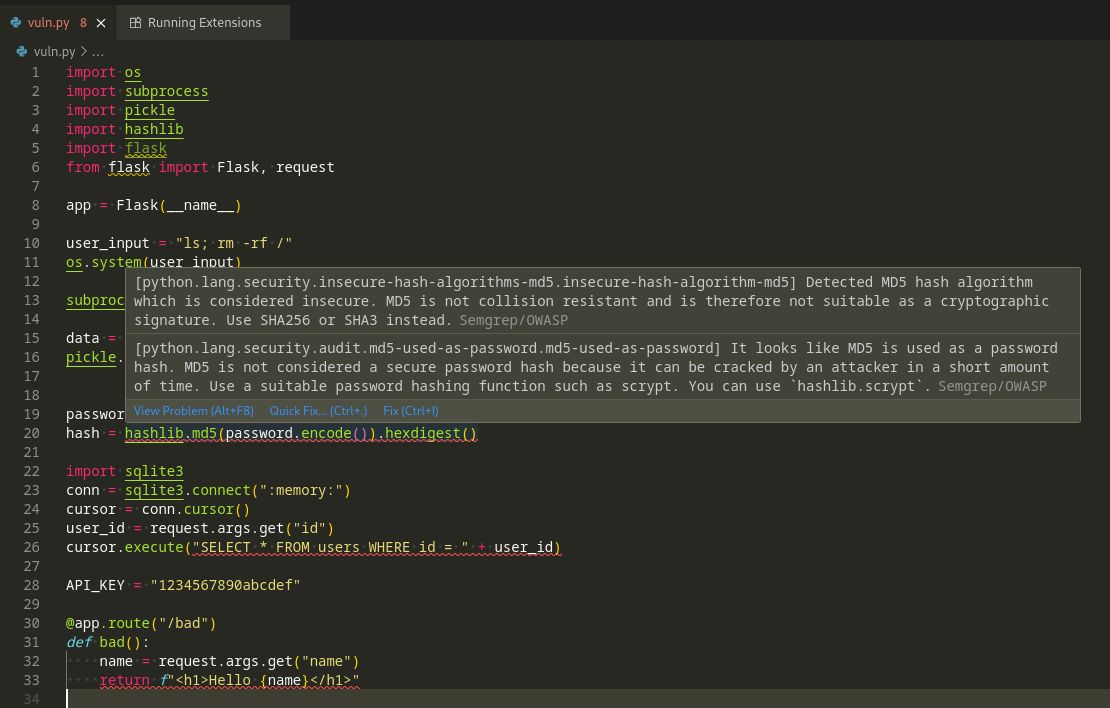
\includegraphics[width=\textwidth]{images/vscode-example.png}
    \caption{Example of the VS Code extension in action.}
    \label{fig:vscode-example}
\end{figure}


\section{Implementation Steps}

The development of the Visual Studio Code extension, "OWASP Guardian", followed a structured process to ensure a robust and user-friendly tool. The key implementation steps are outlined below.

\subsection{Project Setup and Configuration}

The first step was to set up a new VS Code extension project using TypeScript. This involved initializing a new project with the `yo code` command, which generates the basic scaffolding for an extension.

The `package.json` file was then configured to define the extension's metadata, such as its name, description, and activation events. The activation event was set to `onLanguage:python`, which means the extension is activated whenever a Python file is opened.

\begin{minted}{json}
"activationEvents": [
    "onLanguage:python"
],
"contributes": {
    "commands": [
        {
            "command": "vscode-owasp-guardian.scanFile",
            "title": "OWASP Guardian: Scan File"
        }
    ]
},
\end{minted}

\subsection{Activation and Core Components}

The main logic of the extension resides in the `src/extension.ts` file. The `activate` function is the entry point of the extension.

\begin{minted}{ts}
export function activate(context: vscode.ExtensionContext) {
  diagnosticCollection = vscode.languages.createDiagnosticCollection("owaspGuardian");
  context.subscriptions.push(diagnosticCollection);

  const disposable = vscode.commands.registerCommand("owaspGuardian.scanFile", () => {
    const editor = vscode.window.activeTextEditor;
    if (editor) {
      runSemgrep(editor.document);
    }
  });

  context.subscriptions.push(disposable);

  vscode.workspace.onDidSaveTextDocument(doc => runSemgrep(doc));
}
\end{minted}

When activated, the extension creates a `DiagnosticCollection`, which is used to manage and display the diagnostics (i.e., the vulnerability highlights). It also registers a command for manual scanning and an event listener that triggers a scan whenever a document is saved.

\subsection{Integration with Semgrep}

The core of the extension's functionality is its integration with the `semgrep` command-line tool. The `runSemgrep` function is responsible for this integration.

\begin{minted}{typescript}
async function runSemgrep(document: vscode.TextDocument) {
  if (document.languageId !== "python") {
    return;
  }

  try {
    const { stdout } = await pexecFile("semgrep", [
      "--config",
      "p/owasp-top-ten",
      "--json",
      "--quiet",
      document.fileName
    ]);
    // ...
  } catch (err: any) {
    // ...
  }
}
\end{minted}

This function executes `semgrep` as a child process using `child\_process.execFile`. The command is configured to use the OWASP Top 10 ruleset and to output the results in JSON format.

\subsection{Processing and Displaying Results}

The JSON output from `semgrep` is parsed to extract the vulnerability information. For each finding, a `Diagnostic` object is created.

\begin{minted}{typescript}
const result = JSON.parse(stdout);
const diagnostics: vscode.Diagnostic[] = [];

for (const finding of result.results || []) {
  const start = new vscode.Position(finding.start.line - 1, finding.start.col - 1);
  const end = new vscode.Position(finding.end.line - 1, finding.end.col);
  const range = new vscode.Range(start, end);

  const diagnostic = new vscode.Diagnostic(
    range,
    `[${finding.check_id}] ${finding.extra.message}`,
    vscode.DiagnosticSeverity.Error
  );

  diagnostic.source = "Semgrep/OWASP";
  diagnostics.push(diagnostic);
}

diagnosticCollection.set(document.uri, diagnostics);
\end{minted}

The range of the diagnostic is set to match the location of the vulnerability in the code. The severity is set to `Error`, which results in a red highlight. Finally, the diagnostics are added to the `diagnosticCollection`, which makes them visible in the editor. If `semgrep` fails, an error message is shown to the user.

\begin{minted}{typescript}
  } catch (err: any) {
    console.error("Semgrep failed:", err.message || err);
    vscode.window.showErrorMessage(`Semgrep failed: ${err.message || err}`);
  }
\end{minted}

\subsection{Deactivation}

The `deactivate` function is called when the extension is deactivated. It disposes the `diagnosticCollection` to clean up the resources.

\begin{minted}{typescript}
export function deactivate() {
  if (diagnosticCollection) {
    diagnosticCollection.dispose();
  }
}
\end{minted}